%!TEX root = ../../../report.tex
\section{Comparison of simulators} % (fold)
\label{sec:sim_comparison_of_simulators}
When choosing a simulation platform there are several factors to have into account.
Three robotic simulators have been analyzed and compared. 
These are: LPZ Robots \cite{lpzrobots} (see Figure \ref{fig:lpzrobots_example}), V-Rep \cite{vrep} (see Figure \ref{fig:vrep_example}) and Gazebo \cite{gazebo} (see Figure \ref{fig:gazebo_example}).
Some comparisons can be found in the literature as \cite{nogueiracomparative} or \cite{staranowicz2011survey} however the predominant reason has been the integration with ROS.

\begin{figure}[hb!]
  \begin{subfigure}{.33\textwidth}
    \centering
    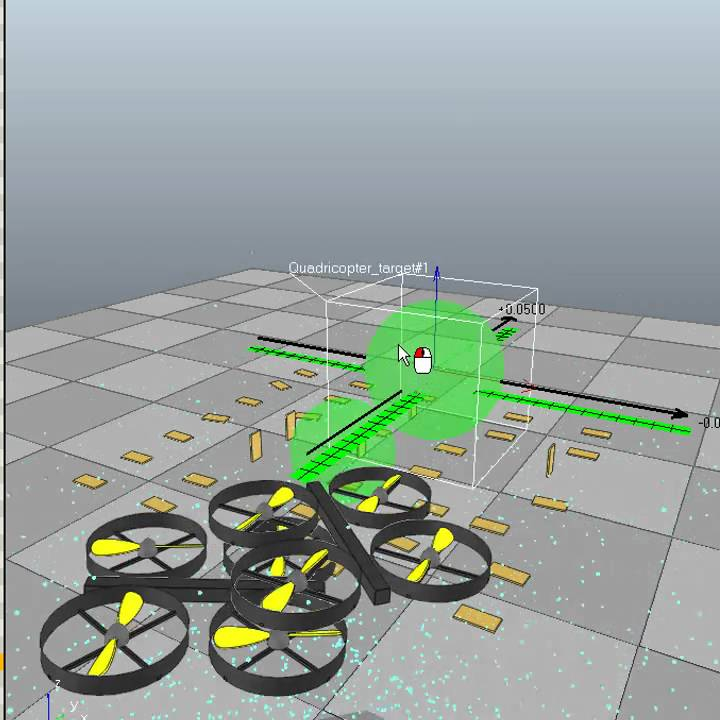
\includegraphics[width=.95\linewidth]{figures/vrep_example}
    \caption{V-Rep example}
    \label{fig:vrep_example}
  \end{subfigure}%
  \begin{subfigure}{.33\textwidth}
    \centering
    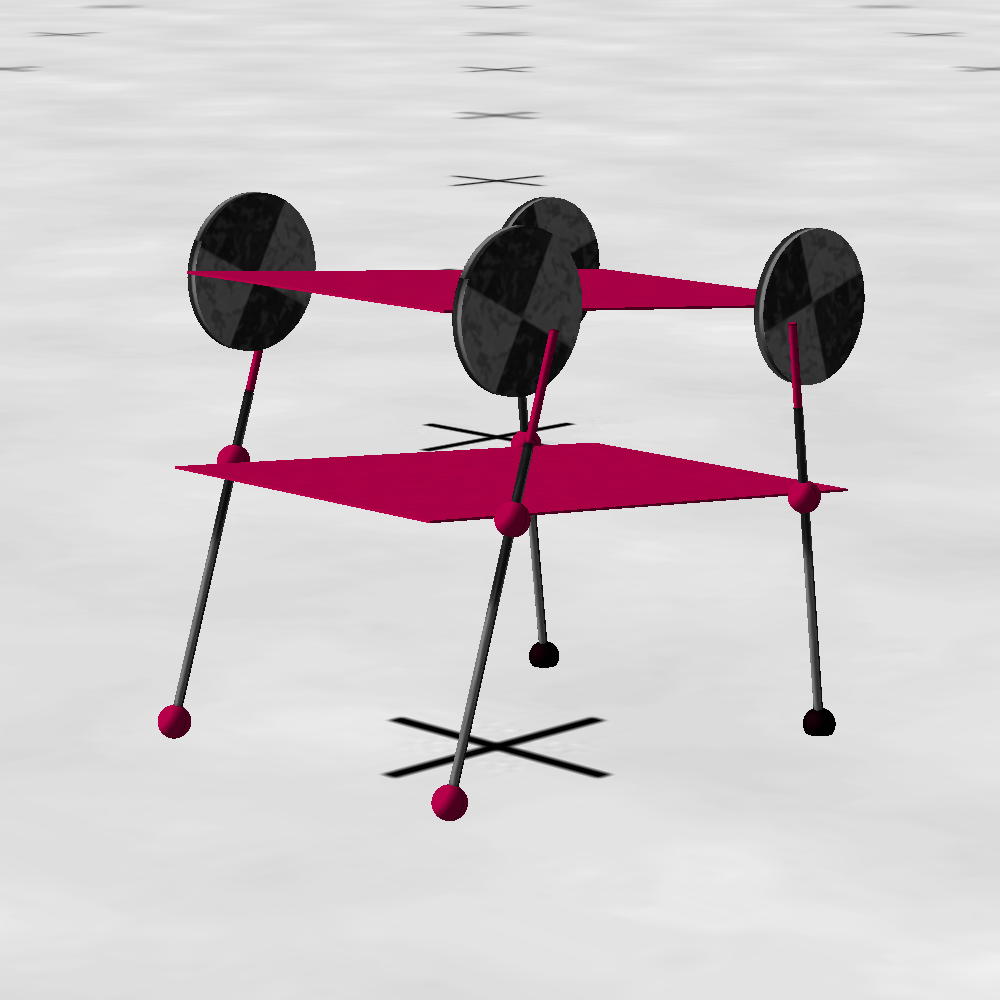
\includegraphics[width=.95\linewidth]{figures/lpzrobots_example}
    \caption{LPZ Robots example}
    \label{fig:lpzrobots_example}
  \end{subfigure}
  \begin{subfigure}{.33\textwidth}
    \centering
    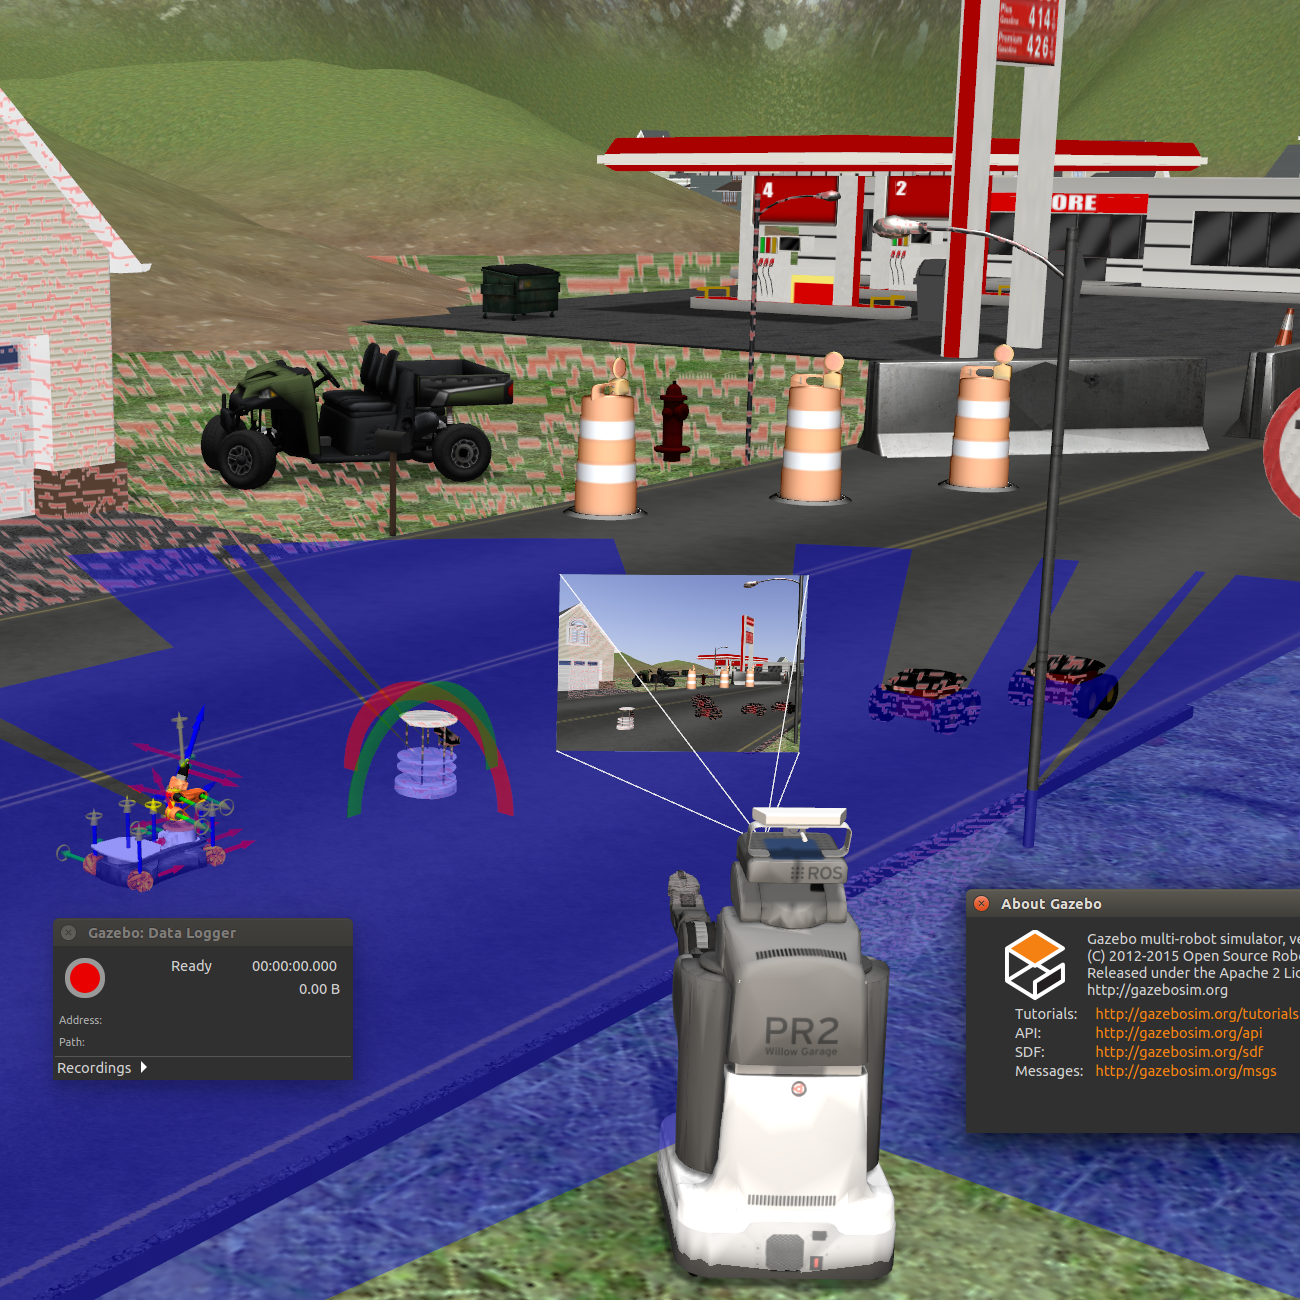
\includegraphics[width=.95\linewidth]{figures/gazebo_example}
    \caption{Gazebo}
    \label{fig:gazebo_example}
  \end{subfigure}
  \caption{Simulation examples of the software analyzed}
  \label{fig:simulation_comparison}
\end{figure}

The device is mainly targeted to be used in the AI department at the Maersk Mc-Kinney Møller Institute, where the toolbox GoRobots is developed.
This is a set of tools, from neuronal networks to genetic algorithms, written in C++ than are supposed to be simulator-independent.
In order to achieve the first condition of reducing the effort of the user when switching from the simulation to real life, ROS \cite{ros} has been used as the software toolbox.
The whole set of tools provided along with its easy extendability give the opportunity to use the controllers developed with GoRobots in both platforms.

Despite all three simulators have a C++ interface that would allow to interface with ROS, in it there is already a simulation integrated: Gazebo.
This reduces the learning curve of the new user and the installation process is easier due to it is included in the Open Source Robotics Foundation (OSRF) repositories.

Regarding the second condition, Gazebo has the feature of change the physics engine in the beginning of the simulation, has multiphysics support (fluids, electromagnetism...), it allows to load external geometries from STL or Collada and, the most important, has an active community behind it providing support and documentation. These are the reasons for taking Gazebo as the simulator for the platform.

In \cite{physics_engine_gazebo_comparison}, a comparison with the different physical engines is carried out.
In the name of simplicity the default one, Open Dynamics Engine (ODE), has been used, though the others have been tested.

% section comparison_of_simulators (end)\[